\chapter{模擬與評估系統表現}
\label{chp:4}

\begin{figure}[ht]
    \centering
    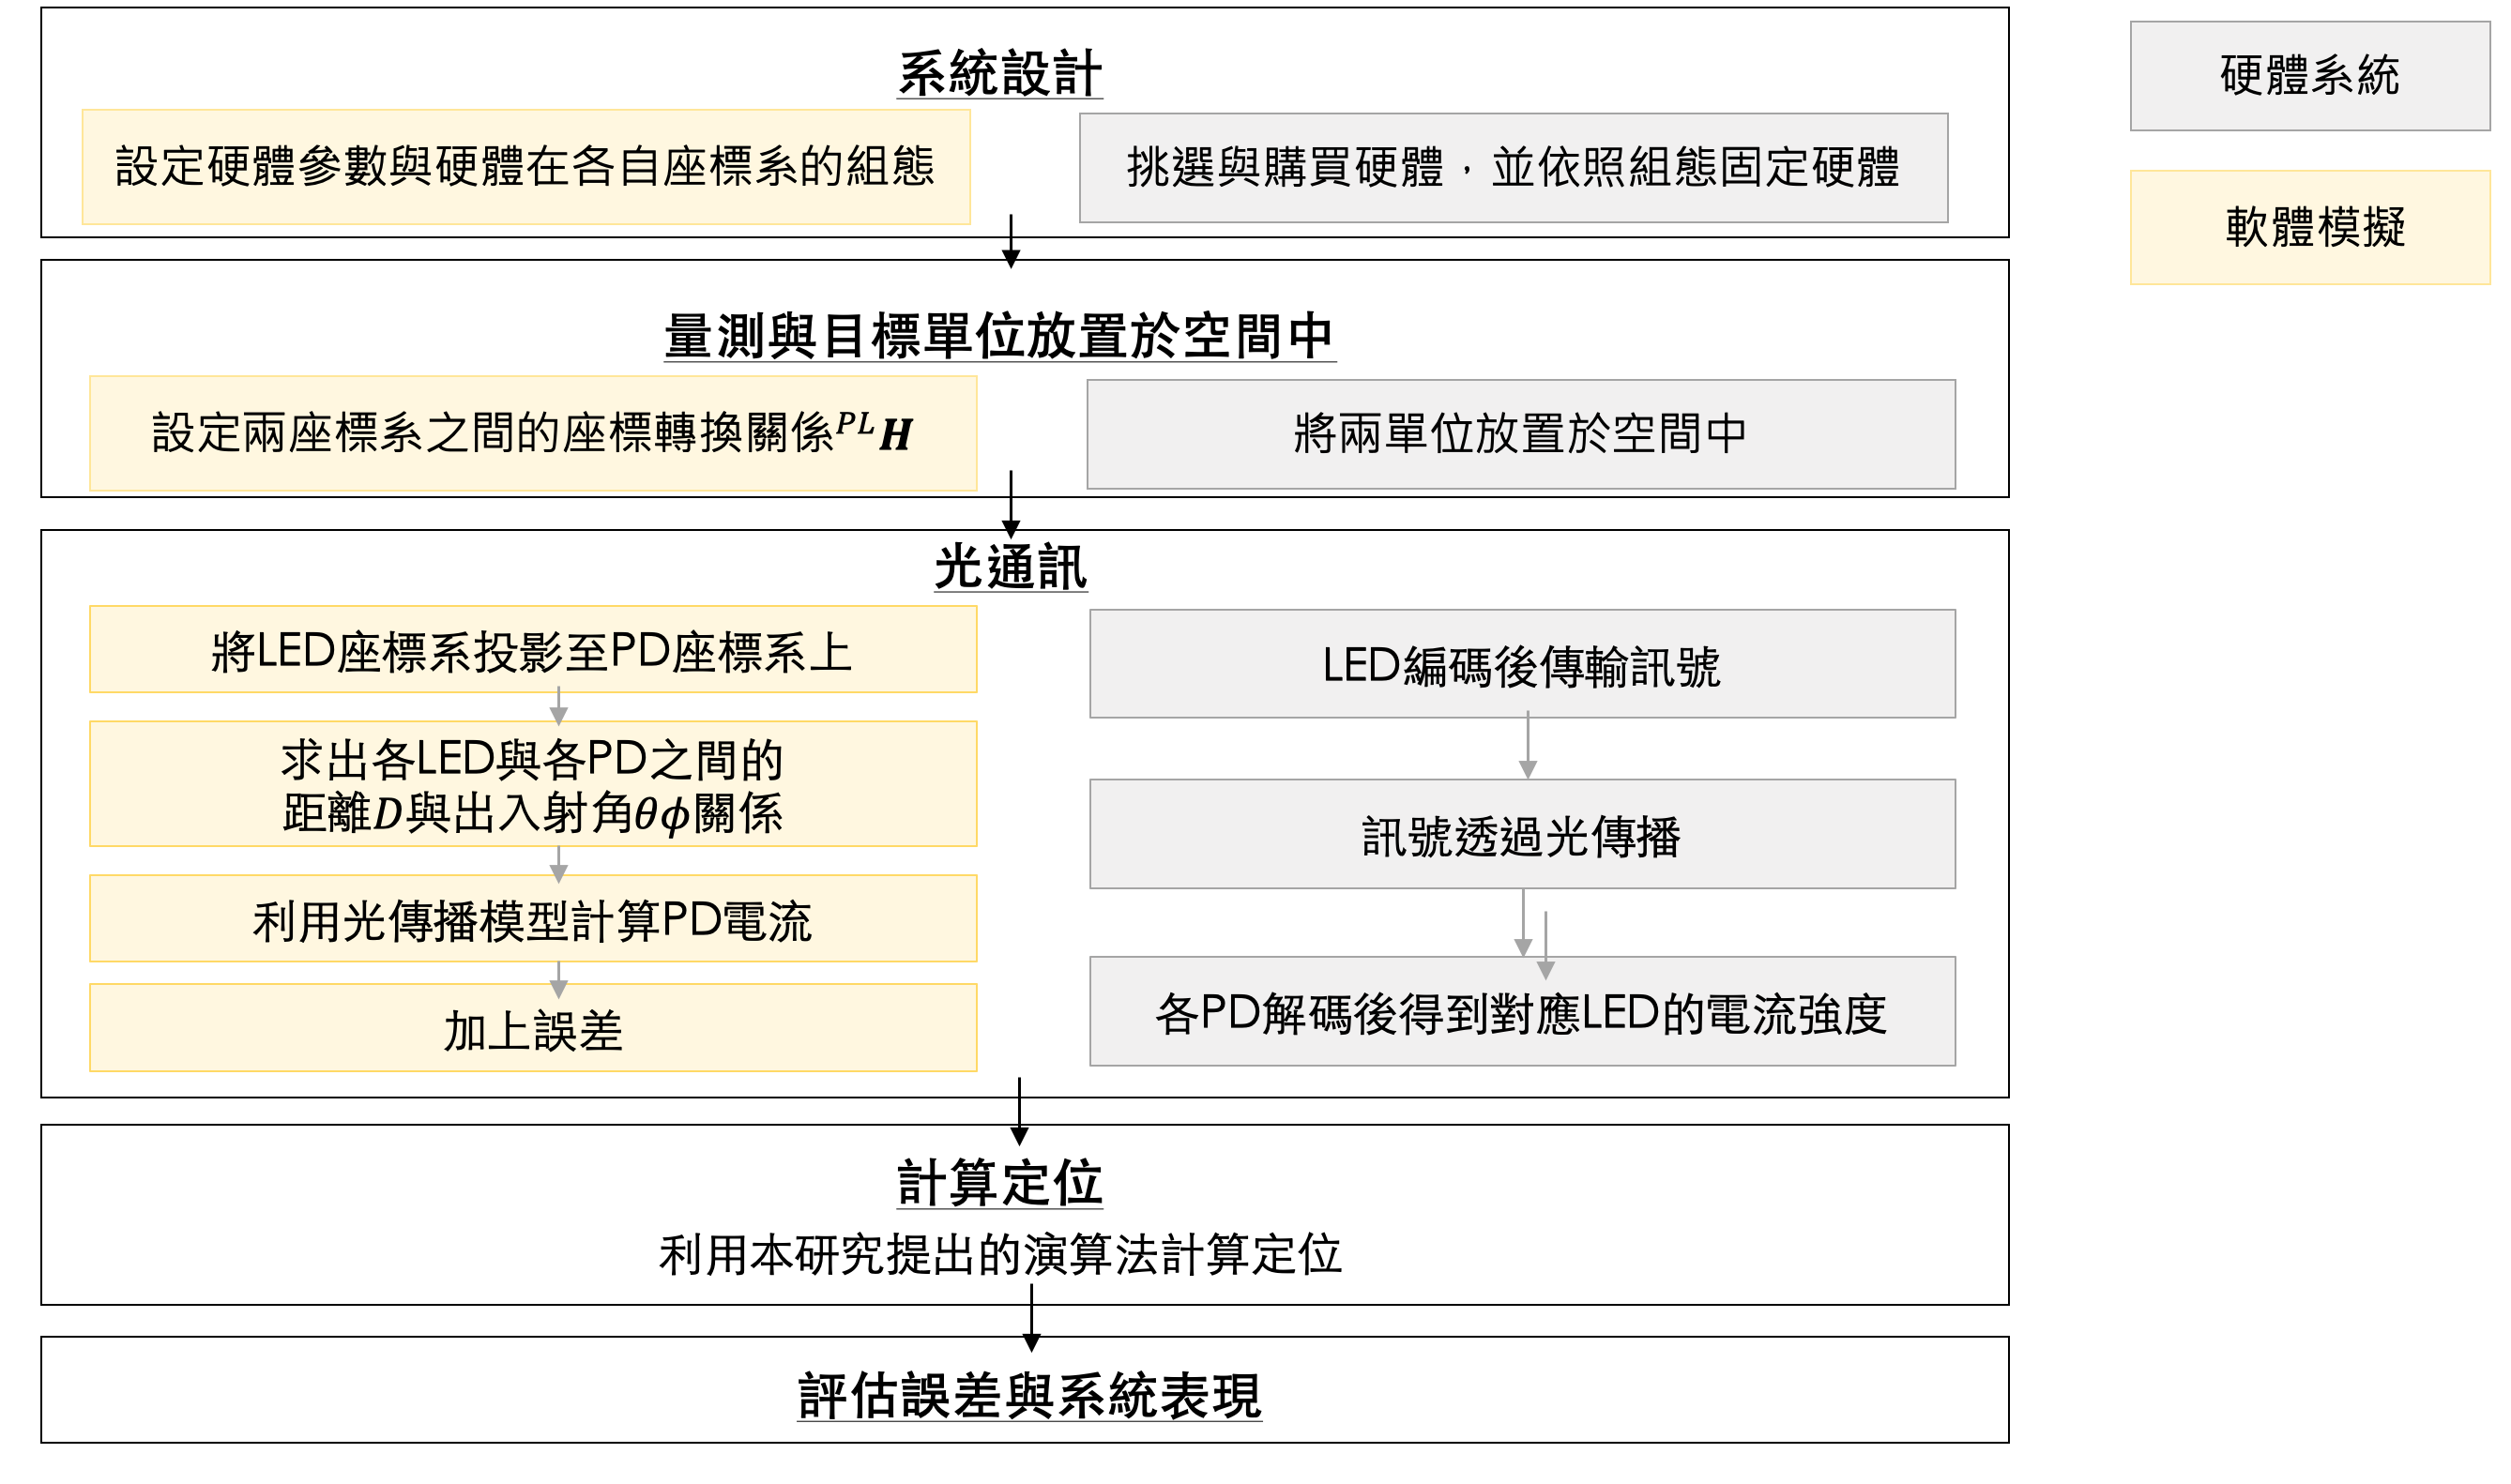
\includegraphics[width=15cm]{ch4pic/simulate_hardware.png}
    \caption{多LED對多PD定位系統以硬體驗證與軟體模擬的流程圖}
    \label{pic:simulate_hardware}
\end{figure}

第三章中,我們提出了一個多LED對多PD系統的演算法,具有獲得三維定位以及目標物姿態的能力,且不需限制目標平面與使用者平面平行,在硬體擺放的指向以及數量上也具有靈活度。而定位演算法的表現,通常會透過架設硬體系統來進行驗證,定位系統的流程可參考圖\ref{pic:simulation_flow}。然而在光通訊發展並不如無線電波段成熟的情況下,架設光通訊系統具有難度,無法直接購買到包裝完整的光通訊套件。因此,大多數的文獻上會透過軟體模擬,建立一虛擬環境將LED與PD系統放至於空間中,將光通訊解碼後的強度資訊模擬輸出,提供給定位演算法計算出相對位置,再針對解出的相對位置誤差對系統表現進行評估。

本章節便會利用軟體模擬的方法,建立一模擬環境,將光通訊的步驟在模擬中完成,再以第三章提出的定位演算法計算出相對位置,並評估誤差與系統表現。以下依序在\ref{chp:simulation}章中詳細介紹模擬方法,並再\ref{chp:scenario}章中介紹模擬的情境,而模擬的結果與分析於\ref{chp:system_perform}章中分析,最後於\ref{chp:4_conclusion}章中總結。

% --------------------------------------
\section{模擬方法}
\label{chp:simulation}

為了針對不同使用情境評估系統表現,模擬流程整理於圖\ref{pic:simulation_flow},其中,由於在評估系統時,需要對不同的使用情境進行設計,因此我們的模擬流程由定義使用情境開始,參考\ref{chp:scenario}章,而根據不同使用情境,量測與目標單位於空間中的相對位置與姿態也會有所不同。系統設計的部分於\ref{chp:hardware_design}章中介紹,需決定的部分包含硬體數量、硬體參數以及硬體組態。有了硬體組態與座標轉換關係,即可透過式\ref{eqn:model_coor_extend}計算出相對位置,如何模擬硬體誤差則在\ref{chp:hardware_error}章中介紹。最後則是透過第三章提出的演算法,計算出相對位置與誤差。


\begin{figure}[ht]
    \centering
    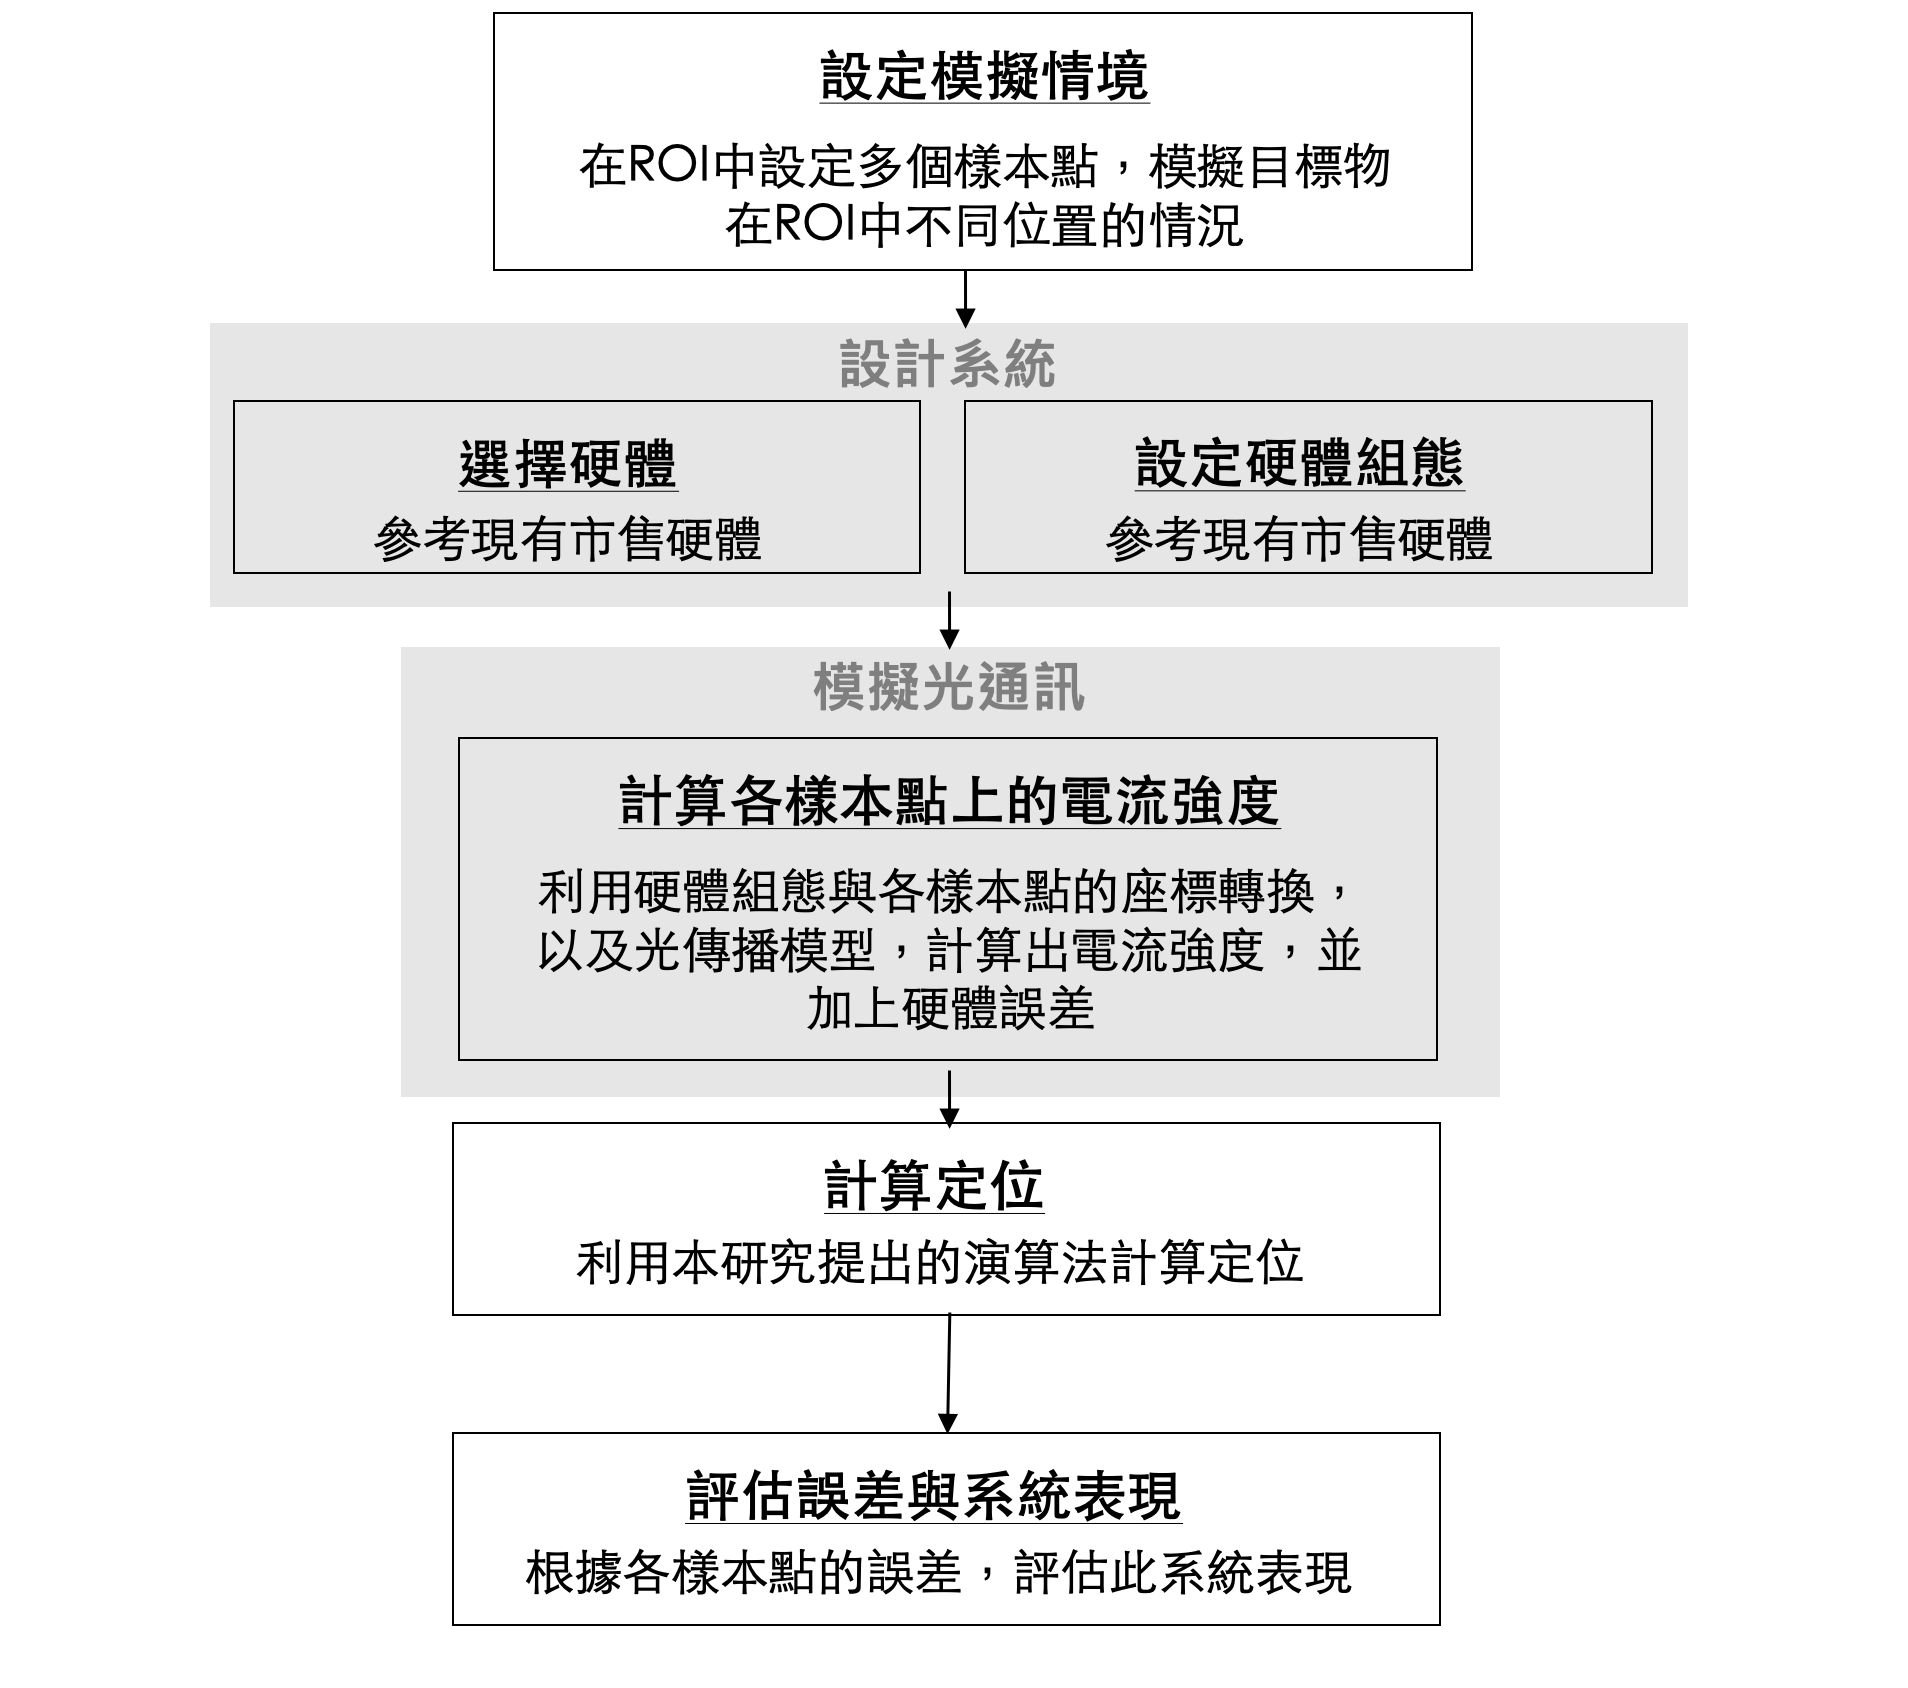
\includegraphics[width=13cm]{ch4pic/simulation_flow.png}
    \caption{模擬流程圖}
    \label{pic:simulation_flow}
\end{figure}

\subsection{定義模擬情境}
\label{chp:scenario}

為了針對不同使用情境評估系統表現,我們於此情境中的感興趣區域(Region of Interest,以下簡稱ROI)中建立多個樣本點,針對第$k$個樣本點中量測出的相對位置$\hat{^{PL}_{k}\boldsymbol{T}}$,計算出與實際相對位置$^{PL}\boldsymbol{T}$的誤差$_k e$,參考圖\ref{pic:error_show}。其中,ROI是相對PD座標系去作定義,也就是將PD視為固定,定義LED座標系相對於PD座標系的座標轉換關係$^{PL}\boldsymbol{H}$。僅定義LED座標系相對於PD座標系的關係之原因,是因為在不考慮環境障礙物情況下,兩座標系的絕對位置並不重要,僅有相對關係會對相對位置造成影響。

\begin{figure}[ht]
    \centering
    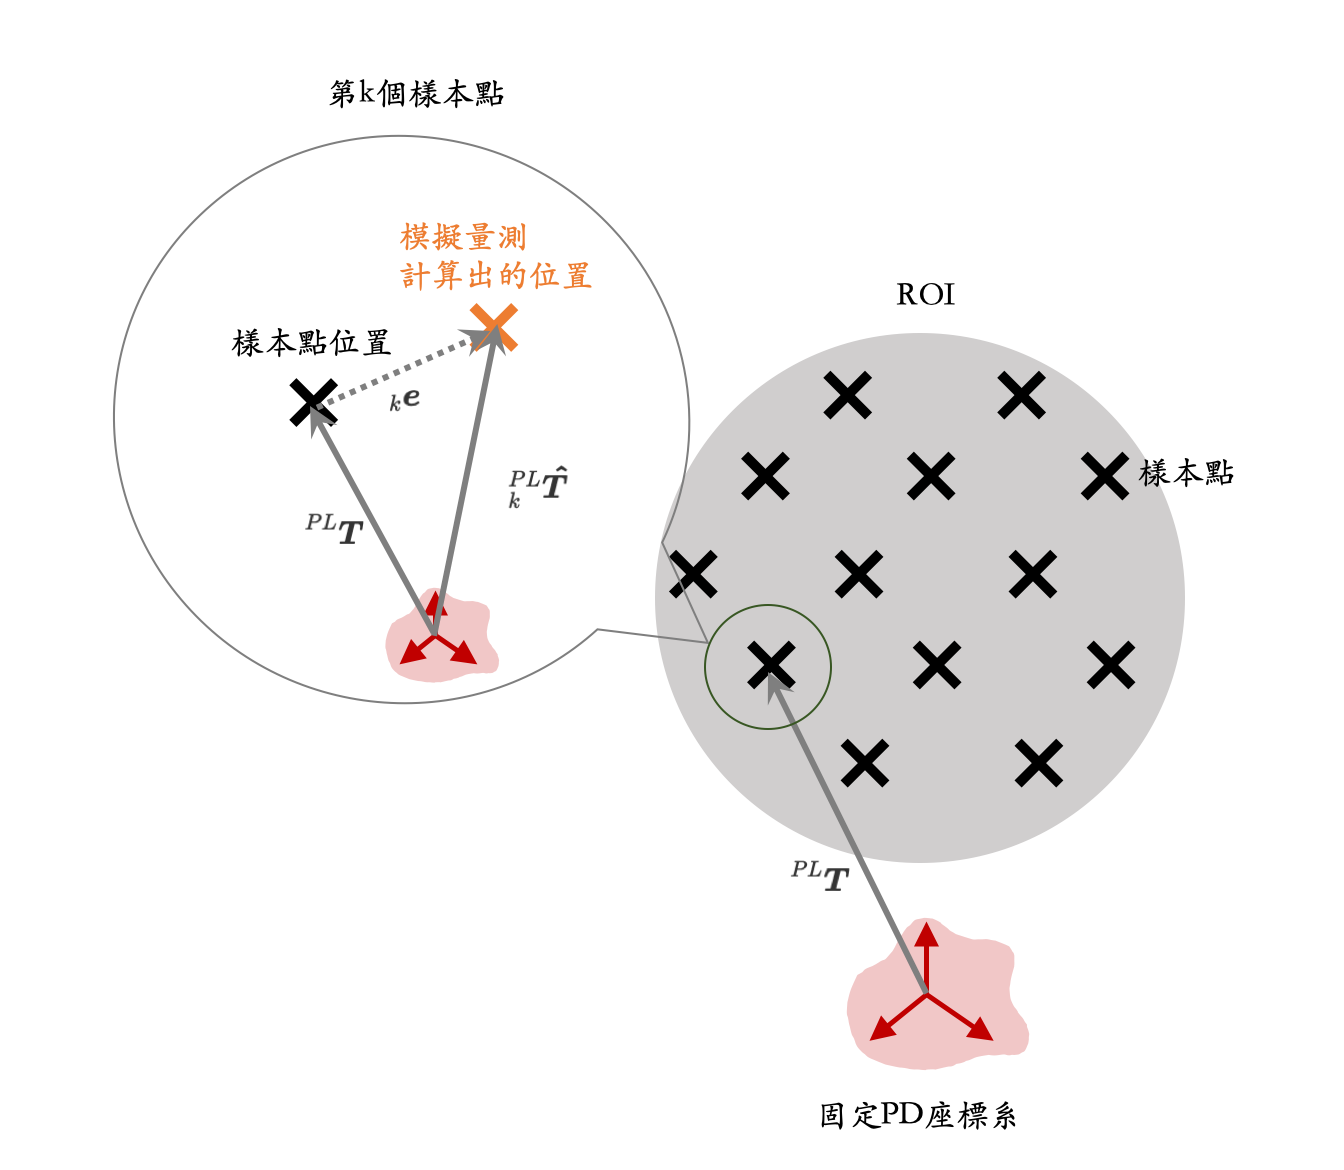
\includegraphics[width=9cm]{ch4pic/error.png}
    \caption{樣本點與誤差}
    \label{pic:error_show}
\end{figure}

在這裡,我們選擇常見的室內定位情境作為模擬情境,也就是目標物LED座標系固定於天花板朝地面照射,而量測者的PD座標系於室內空間中,測試範圍設置的較\cite{case:cart3d}\cite{case:3d_layers}中的都大,為$3 \times 3 \times 3 m$的範圍,如圖\ref{pic:translate_sample}。而由於本研究所使用的演算法並不需限制目標平面與量測平面平行,因此兩座標系之間的姿態也可以改變,除了平移的樣本點還需建立旋轉的樣本點,旋轉樣本點由翻滾(以下稱為Roll)、俯仰(以下稱為Pitch)、偏擺(以下稱為yaw)三個旋轉角度定義,旋轉順序依序為Roll, Pitch, Yaw。旋轉樣本可參考圖\ref{pic:rotate_sample},紅色箭頭代表的是PD座標系Z軸,藍色的各個箭頭則代表與其相對的的LED座標系Z軸,並以極座標圖呈現於圖中。

\begin{figure}[ht]
    \centering
    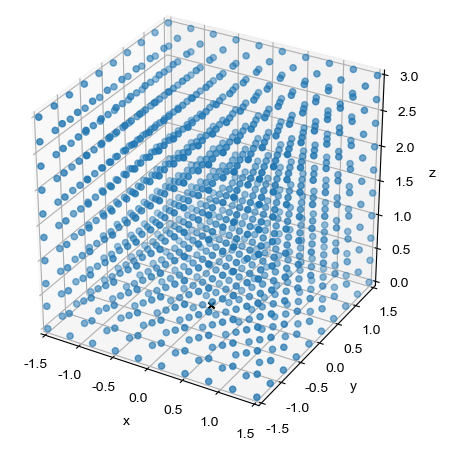
\includegraphics[width=6cm]{ch4pic/translate_sample.png}
    \caption{平移樣本點}
    \label{pic:translate_sample}
\end{figure}

\begin{figure}[ht]
    \centering
    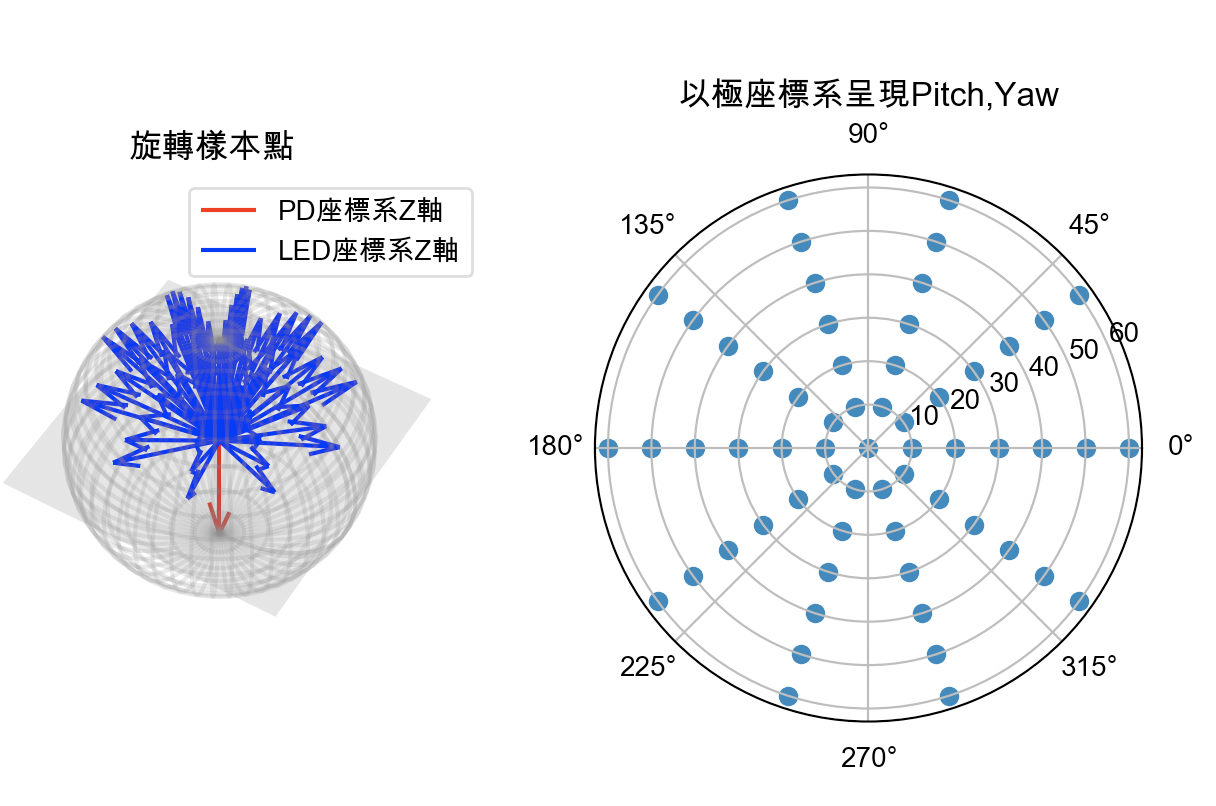
\includegraphics[width=8cm]{ch4pic/rotate_sample.png}
    \caption{旋轉樣本點}
    \label{pic:rotate_sample}
\end{figure}

\begin{table}[h!]
    \begin{center}
      \caption{平移樣本點}
      \label{tab:translate}
      \begin{tabular}{c|c|c|c} % <-- Alignments: 1st column left, 2nd middle and 3rd right, with vertical lines in between
         & \textbf{最小值} & \textbf{最大值}&\textbf{樣本數}\\
        \hline
        $t_x$ & -1.5 & 1.5&10\\
        $t_y$ & -1.5 & 1.5&10\\
        $t_z$ & 0 & 3 &10\\
      \end{tabular}
    \end{center}
  \end{table}

  \begin{table}[h!]
    \begin{center}
      \caption{旋轉樣本點}
      \label{tab:rotate}
      \begin{tabular}{c|c|c|c} % <-- Alignments: 1st column left, 2nd middle and 3rd right, with vertical lines in between
        & \textbf{最小值} & \textbf{最大值}&\textbf{樣本數}\\
       \hline
       Roll & $\pi$ & $\pi$&1\\
       Pitch & $\pi/18$ &$\pi/3$&6\\
       Yaw & $\pi/5$ & $2\pi$&10\\
     \end{tabular}
   \end{center}
 \end{table}

如表\ref{tab:translate}中所示,一共有$10\times 10\times 10$總共一千個平移樣本點,旋轉樣本點則有$1\times 6\times 10$共六十個,兩者相乘代表總共六萬個樣本點。這代表著每個平移樣本點上皆需做出60次旋轉,以旋轉樣本點來看也是,每個旋轉樣本點都需在每個平移樣本點上計算一次。



\subsection{硬體選擇與設計}
\label{chp:hardware_design}

硬體組態的部分,位置的限制如\ref{chp:algorithm_constraint}章中所述,需限制PD擺放位置於PD座標系原點:$^P\boldsymbol{P}_p=
\left[\begin{array}{ccc}0&0&0\end{array}\right]^T$,LED的擺放位置也限制於LED座標系原點:$^L\boldsymbol{P}_l=
\left[\begin{array}{ccc}0&0&0\end{array}\right]^T$。

硬體數量的部分,參考\ref{chp:orient_conclu}章中所述,LED與PD數量各需要最少三個來達成三維定位,因此我們將PD和LED硬體的數量上下限,設計範圍定在三個到十五個之間。

硬體參數的部分,LED參考\cite{datasheet:led_vsma},以供應5A時的輻射強度作參考,取$Pt=1.7\pi W$,而PD則參考\cite{datasheet:BPW},將$Re\times A = 4.2\times10^{-6}$,而兩硬體的朗博次方則都設定為一。


\subsection{誤差模擬方法}
\label{chp:hardware_error}

圖\ref{pic:simulation_flow}流程中,模擬光通訊的部分可透過式\ref{eqn:model_algorithm_filter}獲得,而為了更真實的模擬現實狀況,參考\cite{survey_light2018}中對誤差的模擬,呈現於式\ref{eqn:noise}中,$\hat{Ie}_{lp}$代表第l個LED對第p個PD的量測電流,其組成包含了理想的量測電流$Ie_{lp}$與PD硬體誤差。PD硬體誤差中,又可分為熱雜訊$It$(Thermal Noise)與散粒雜訊$Is$(Shot Noise),各自呈現於式\ref{eqn:thermal_noise}與式\ref{eqn:shot_noise}中,其中$Kb$為波茲曼常數(Boltzmann constant)、$Te$為絕對溫度、$B$為頻寬、$Rs$為分路電阻(Shunt Resistance)、$q$為電子電荷。

\begin{equation}
\label{eqn:noise}
    \hat{Ie}_{lp}=Ie_{lp}+\sqrt{It_{lp}^2+Is_{lp}^2} 
\end{equation}


\begin{gather}
    \label{eqn:thermal_noise}
    It_{lp}=\sqrt{\frac{4 Kb Te B}{Rs}}\\
    \label{eqn:shot_noise}
    Is_{lp}=\sqrt{2qIe_{lp}B}
\end{gather}

% --------------------------------------



% --------------------------------------
\section{評估系統表現}
\label{chp:system_perform}



根據以上設定,我們將六萬個樣本點進行定位,然而,各樣本點都有可能遇到無法求解的狀況,如\ref{chp:orient_conclu}章所提到,若沒有任何一個LED同時將訊號傳送給三個以上的PD,則無法解出方位;而若沒有任何一個PD同時接受到三個以上LED資訊,則無法計算距離。即使我們今天系統設計有超過三個以上的LED與PD硬體數量,在\ref{chp:algorithm_filter}章中也會將訊號過大、過小的數值去除,導致所得訊號不足求解的狀況。在各樣本點可能會解不出來的情況下,解不出來則會完全無法計算誤差,因此無法利用樣本點平均誤差來完整描述系統的表現。

因此,我們改看「在容許範圍$To$(Tolerance)」內的樣本點比例,在這邊我們設定$To=0.1m$,而結果呈現於圖\ref{pic:sample_out}。

\begin{figure}[ht]
    \centering
    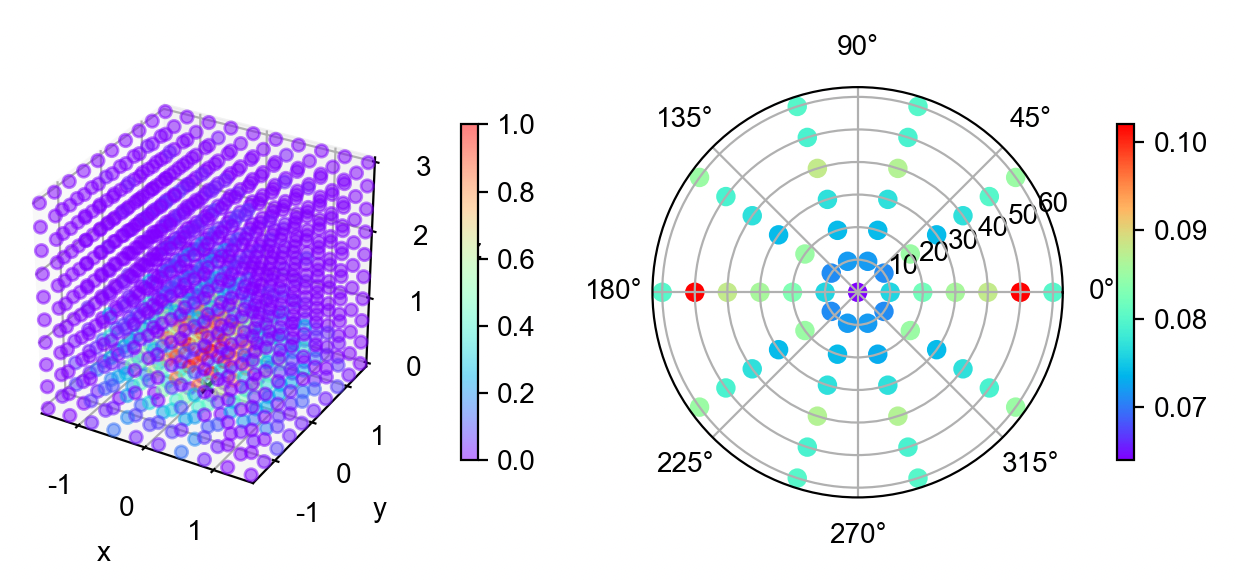
\includegraphics[width=9cm]{ch4pic/sample_out.png}
    \caption{容許範圍內的樣本點比例}
    \label{pic:sample_out}
\end{figure}

觀察圖中的現象,在PD座標系延伸出去,有一橢圓區塊具有很高的定位能力,定位能力的分佈與其他文獻符合。

而由於第三章此演算法並沒有限制硬體數量、朗博次方與硬體指向,在設計上是有靈活度的,因此我們透過改變這幾項變數,來觀察系統的反應。其中,LED與PD指向的部分,我們將每個硬體皆具有的兩個由度限制剩下一個,假設方位角平均分配:$^P\beta_p = 2\pi/P$、$^L\beta_l = 2\pi/L$,仰角的部分則限制必須相同$^P\alpha_p =^P\alpha$、$^L\alpha_l = ^L\alpha$。在這樣的限制下,我們分別探討各項變數的影響。



\subsection{朗博次方的影響}

在假設$^P\alpha_p =\pi/18$、$^L\alpha_l = \pi/18$,以及硬體數量$L=P-8$的情況下,我們改變朗博次方,並將樣本中於容許範圍內的比例,呈現於圖\ref{pic:m_translate}與圖\ref{pic:m_rotate}中。隨著朗博次方的提升,硬體所照射的範圍越來越小,因此容許範圍內比例高的的區域便越顯集中。

\begin{figure}[h!]
    \centering
    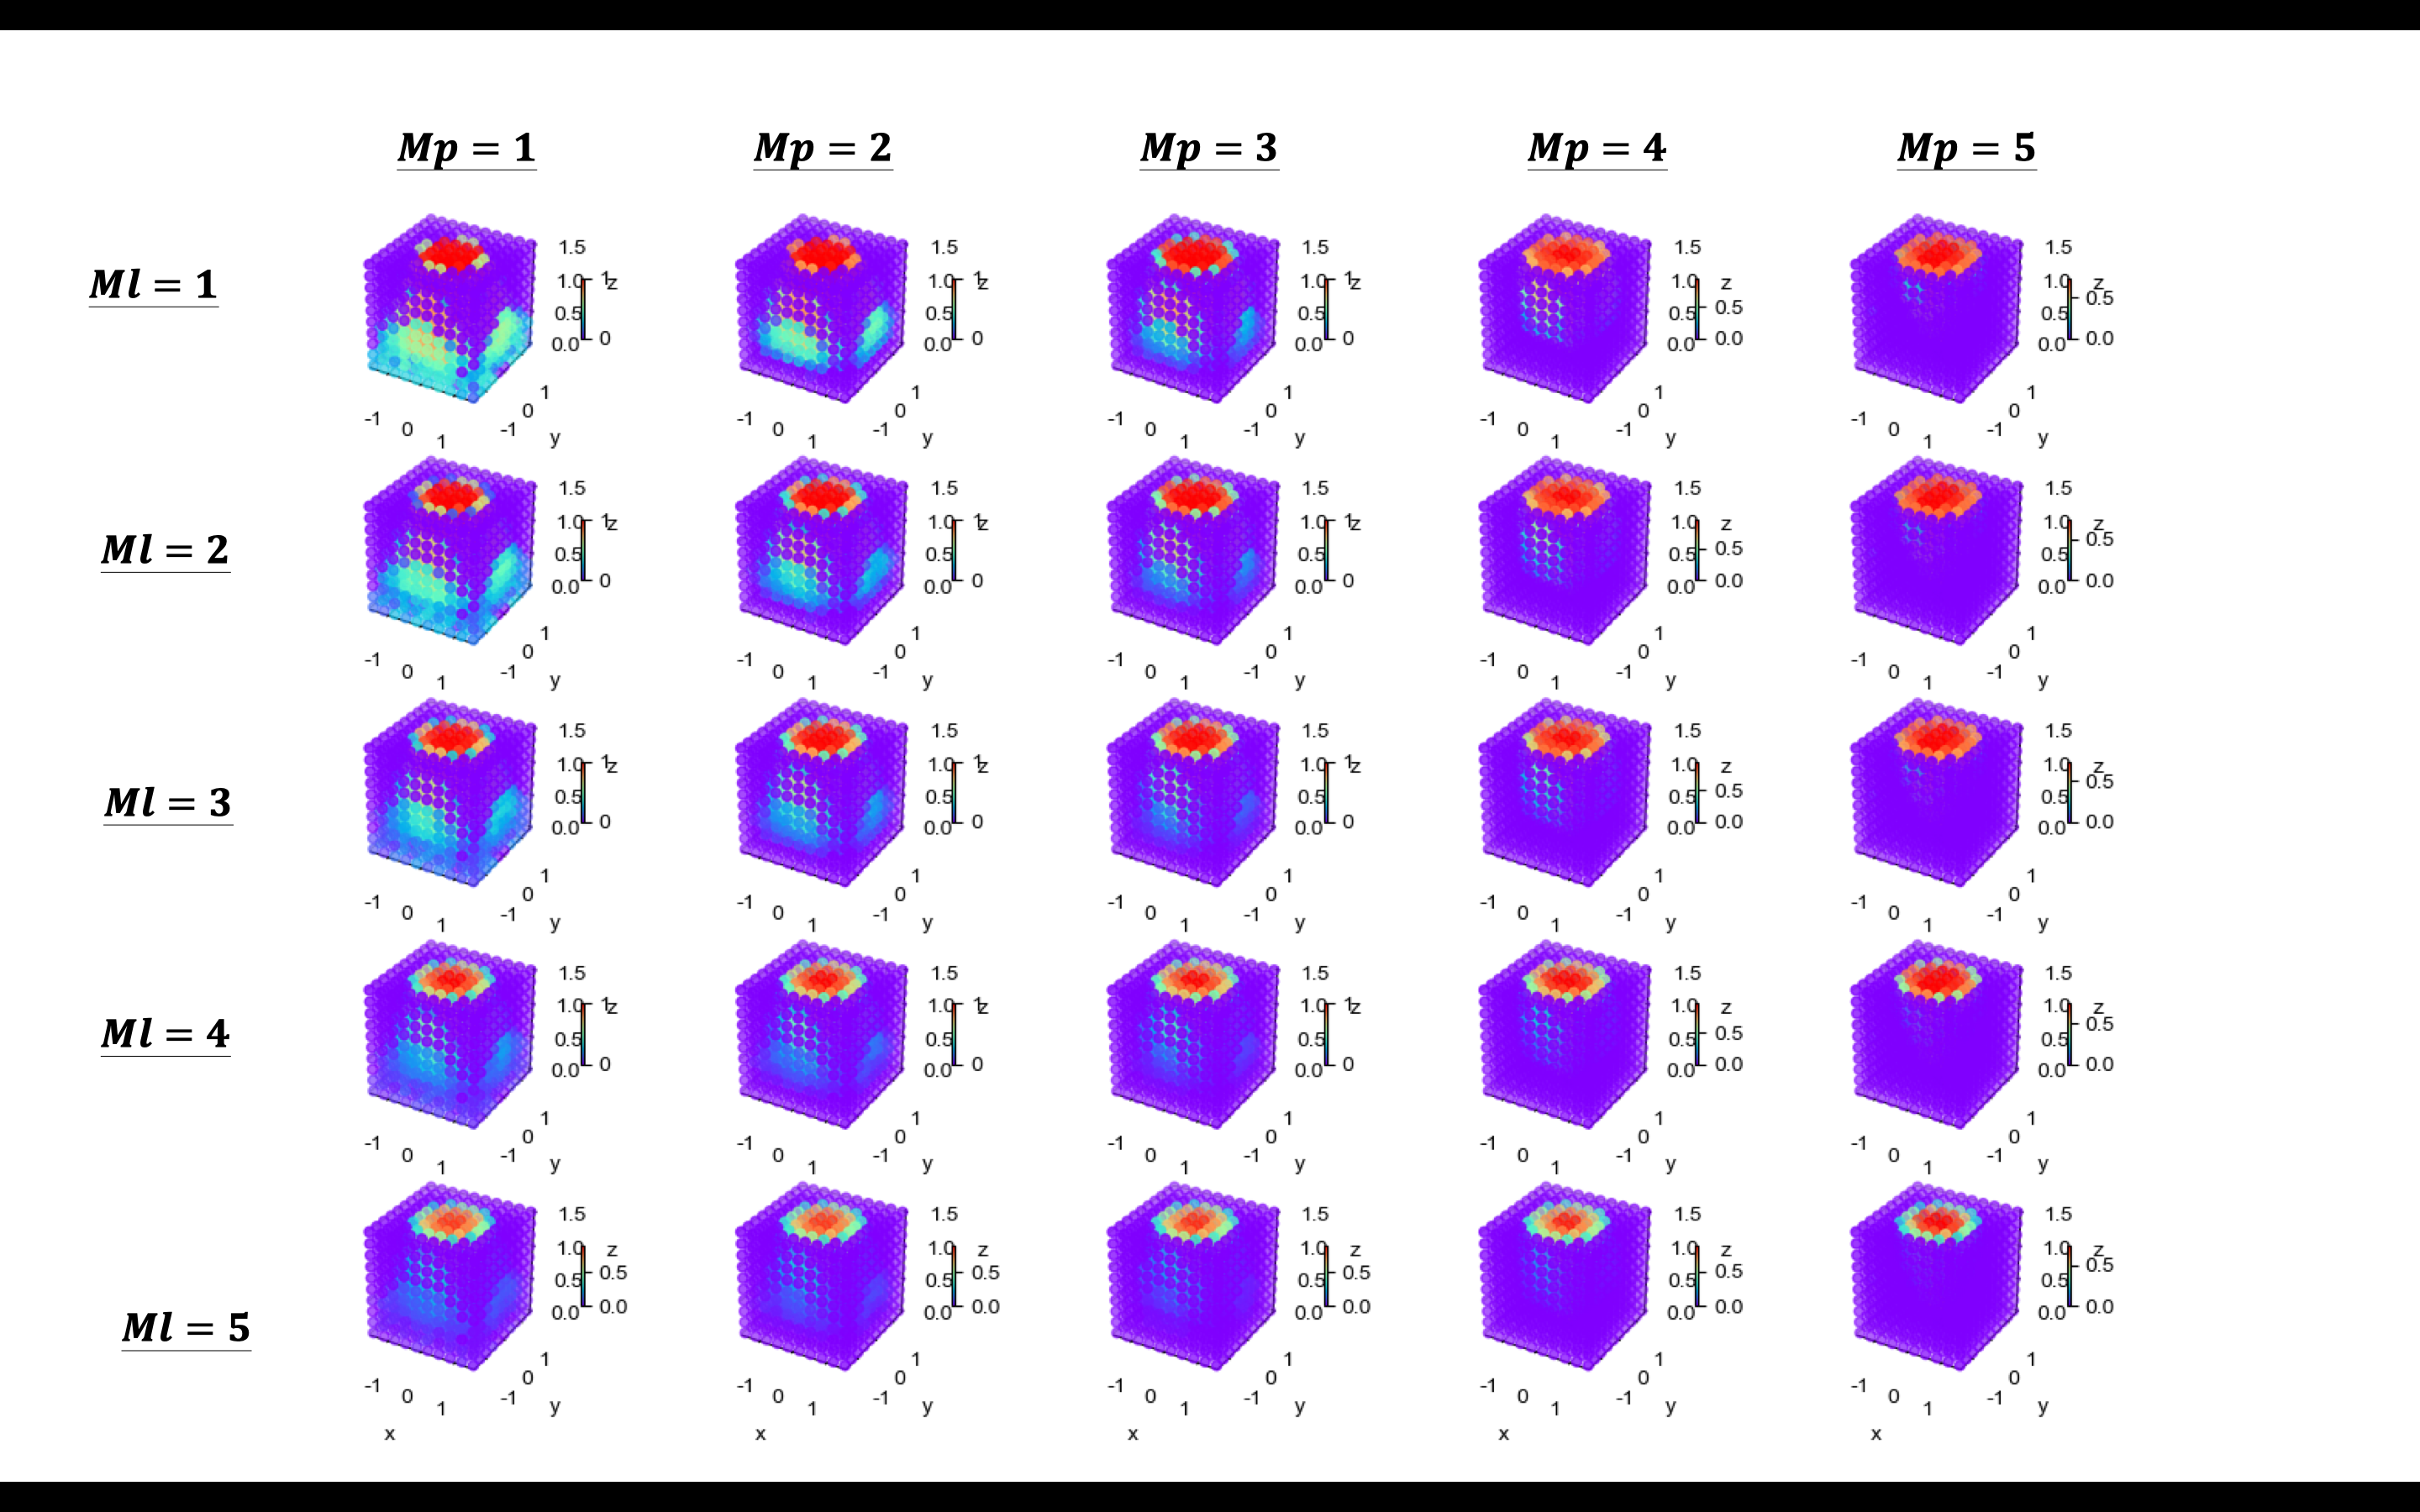
\includegraphics[width=14cm]{ch4pic/m_translate.png}
    \caption{改變朗博次方對平移樣本點的影響}
    \label{pic:m_translate}
\end{figure}
\begin{figure}[h!]
    \centering
    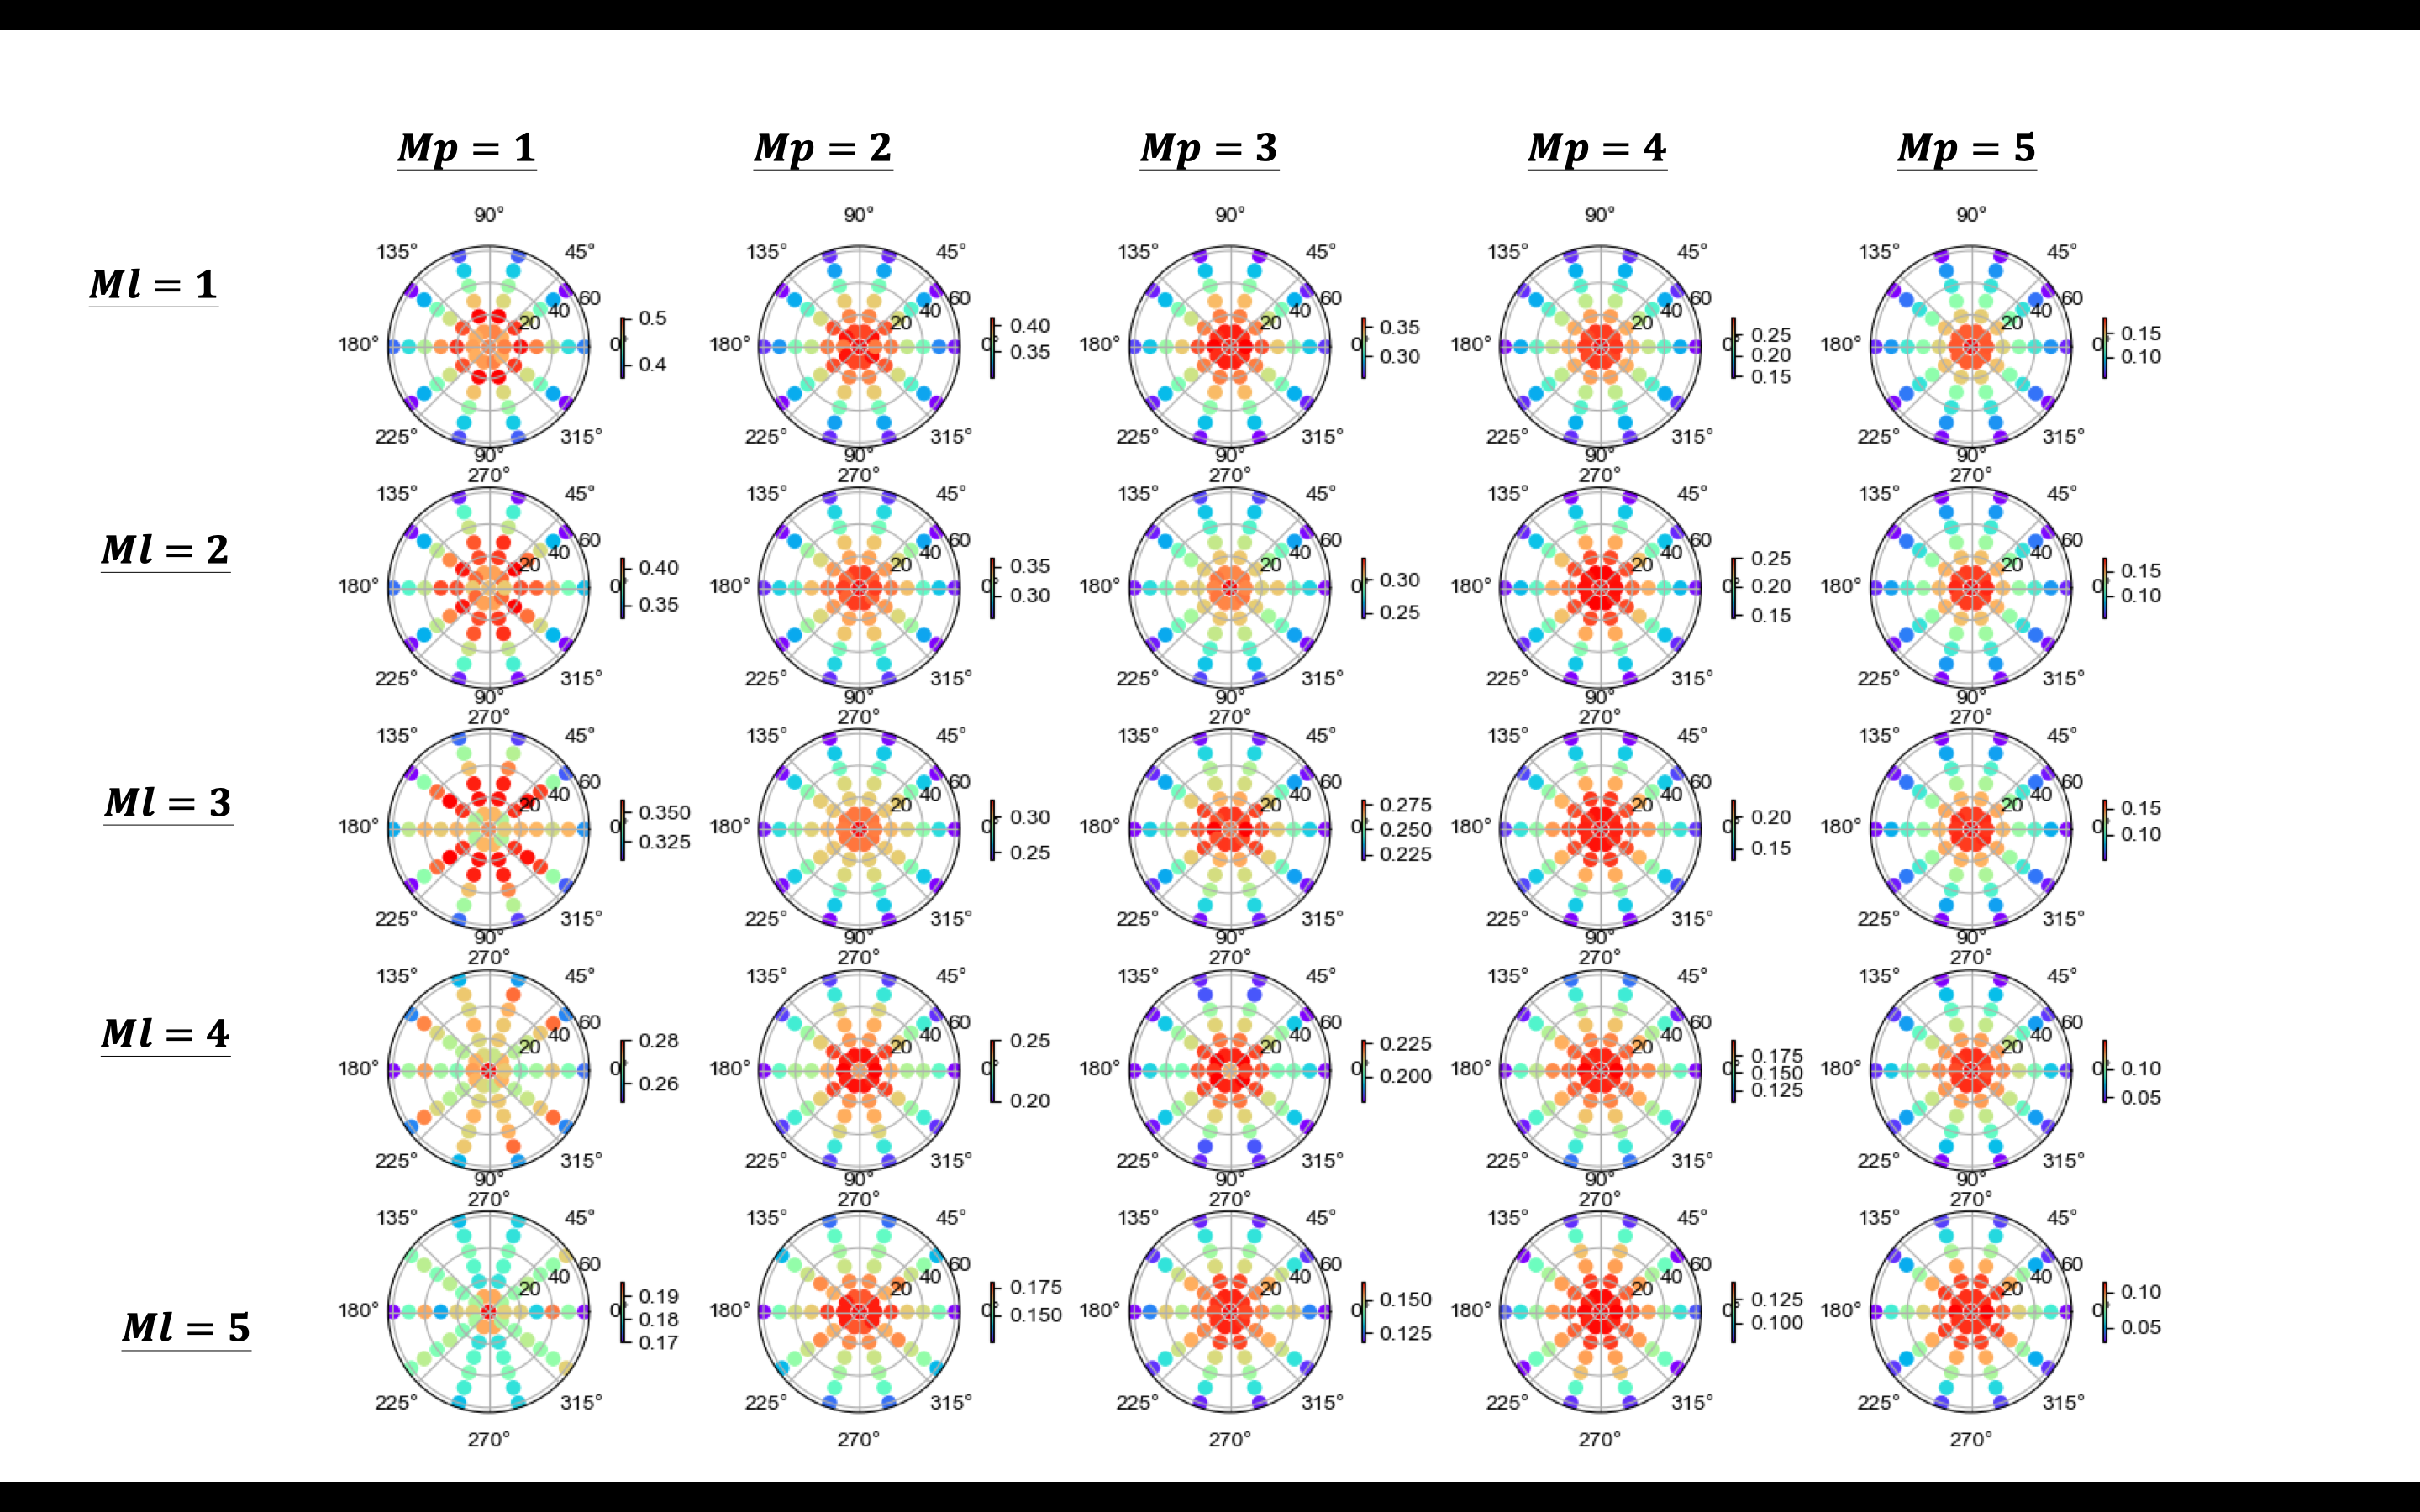
\includegraphics[width=14cm]{ch4pic/m_rotate.png}
    \caption{改變朗博次方對旋轉樣本點的影響}
    \label{pic:m_rotate}
\end{figure}

我們將平移與旋轉樣本點總共六萬個點中,在容許範圍內的比例,呈現於圖\ref{pic:m_effect},我們可以觀察到在此情境中,較小的朗博次方使系統表現較佳。

\begin{figure}[h!]
    \centering
    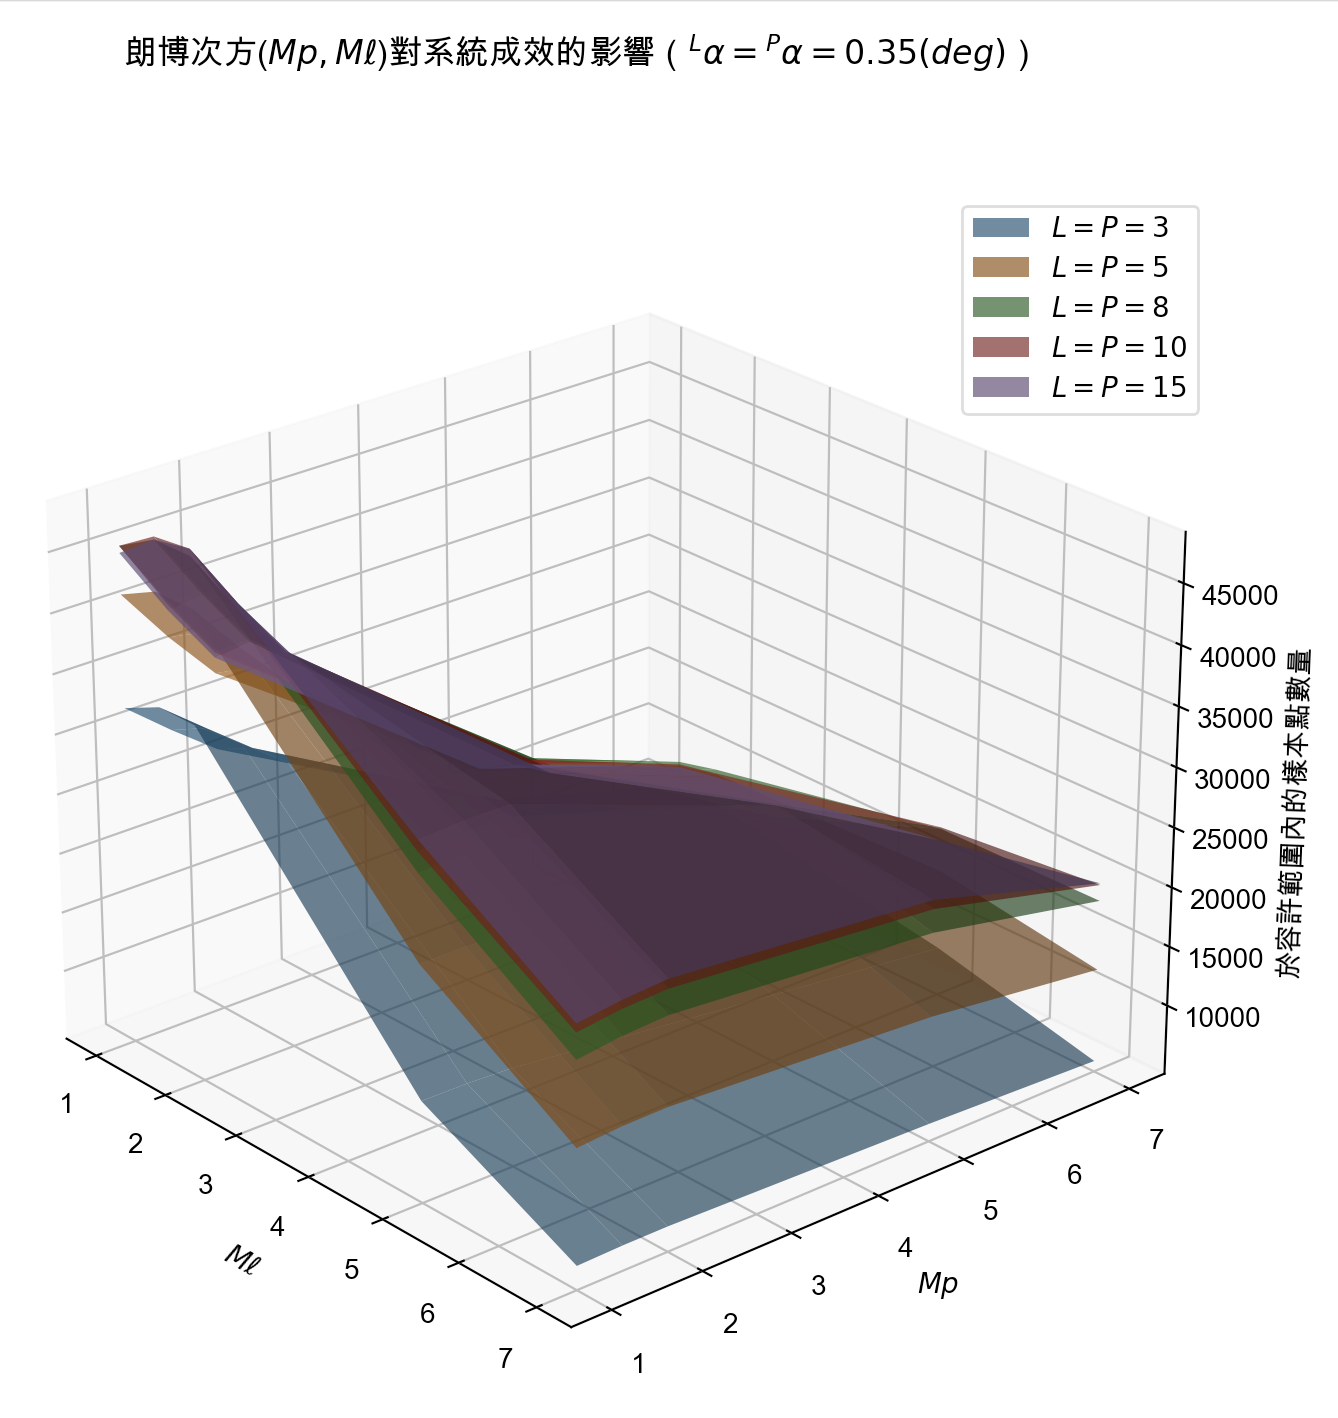
\includegraphics[width=9cm]{ch4pic/m_effect.png}
    \caption{改變朗博次方對系統的影響}
    \label{pic:m_effect}
\end{figure}



\subsection{LED與PD指向的影響}

在假設朗博次方$Mp=M\ell=1$,以及硬體數量$L=P-8$的情況下,我們改變硬體指向$^P\alpha,^L\alpha$,並將樣本中於容許範圍內的比例,呈現於圖\ref{pic:alpha_translate}與圖\ref{pic:alpha_rotate}中。隨著硬體指向提升,多個硬體之間重疊的覆蓋範圍便越來越小,漸漸僅剩下於中心位置的樣本點:$x,y,=0$。

\begin{figure}[h!]
    \centering
    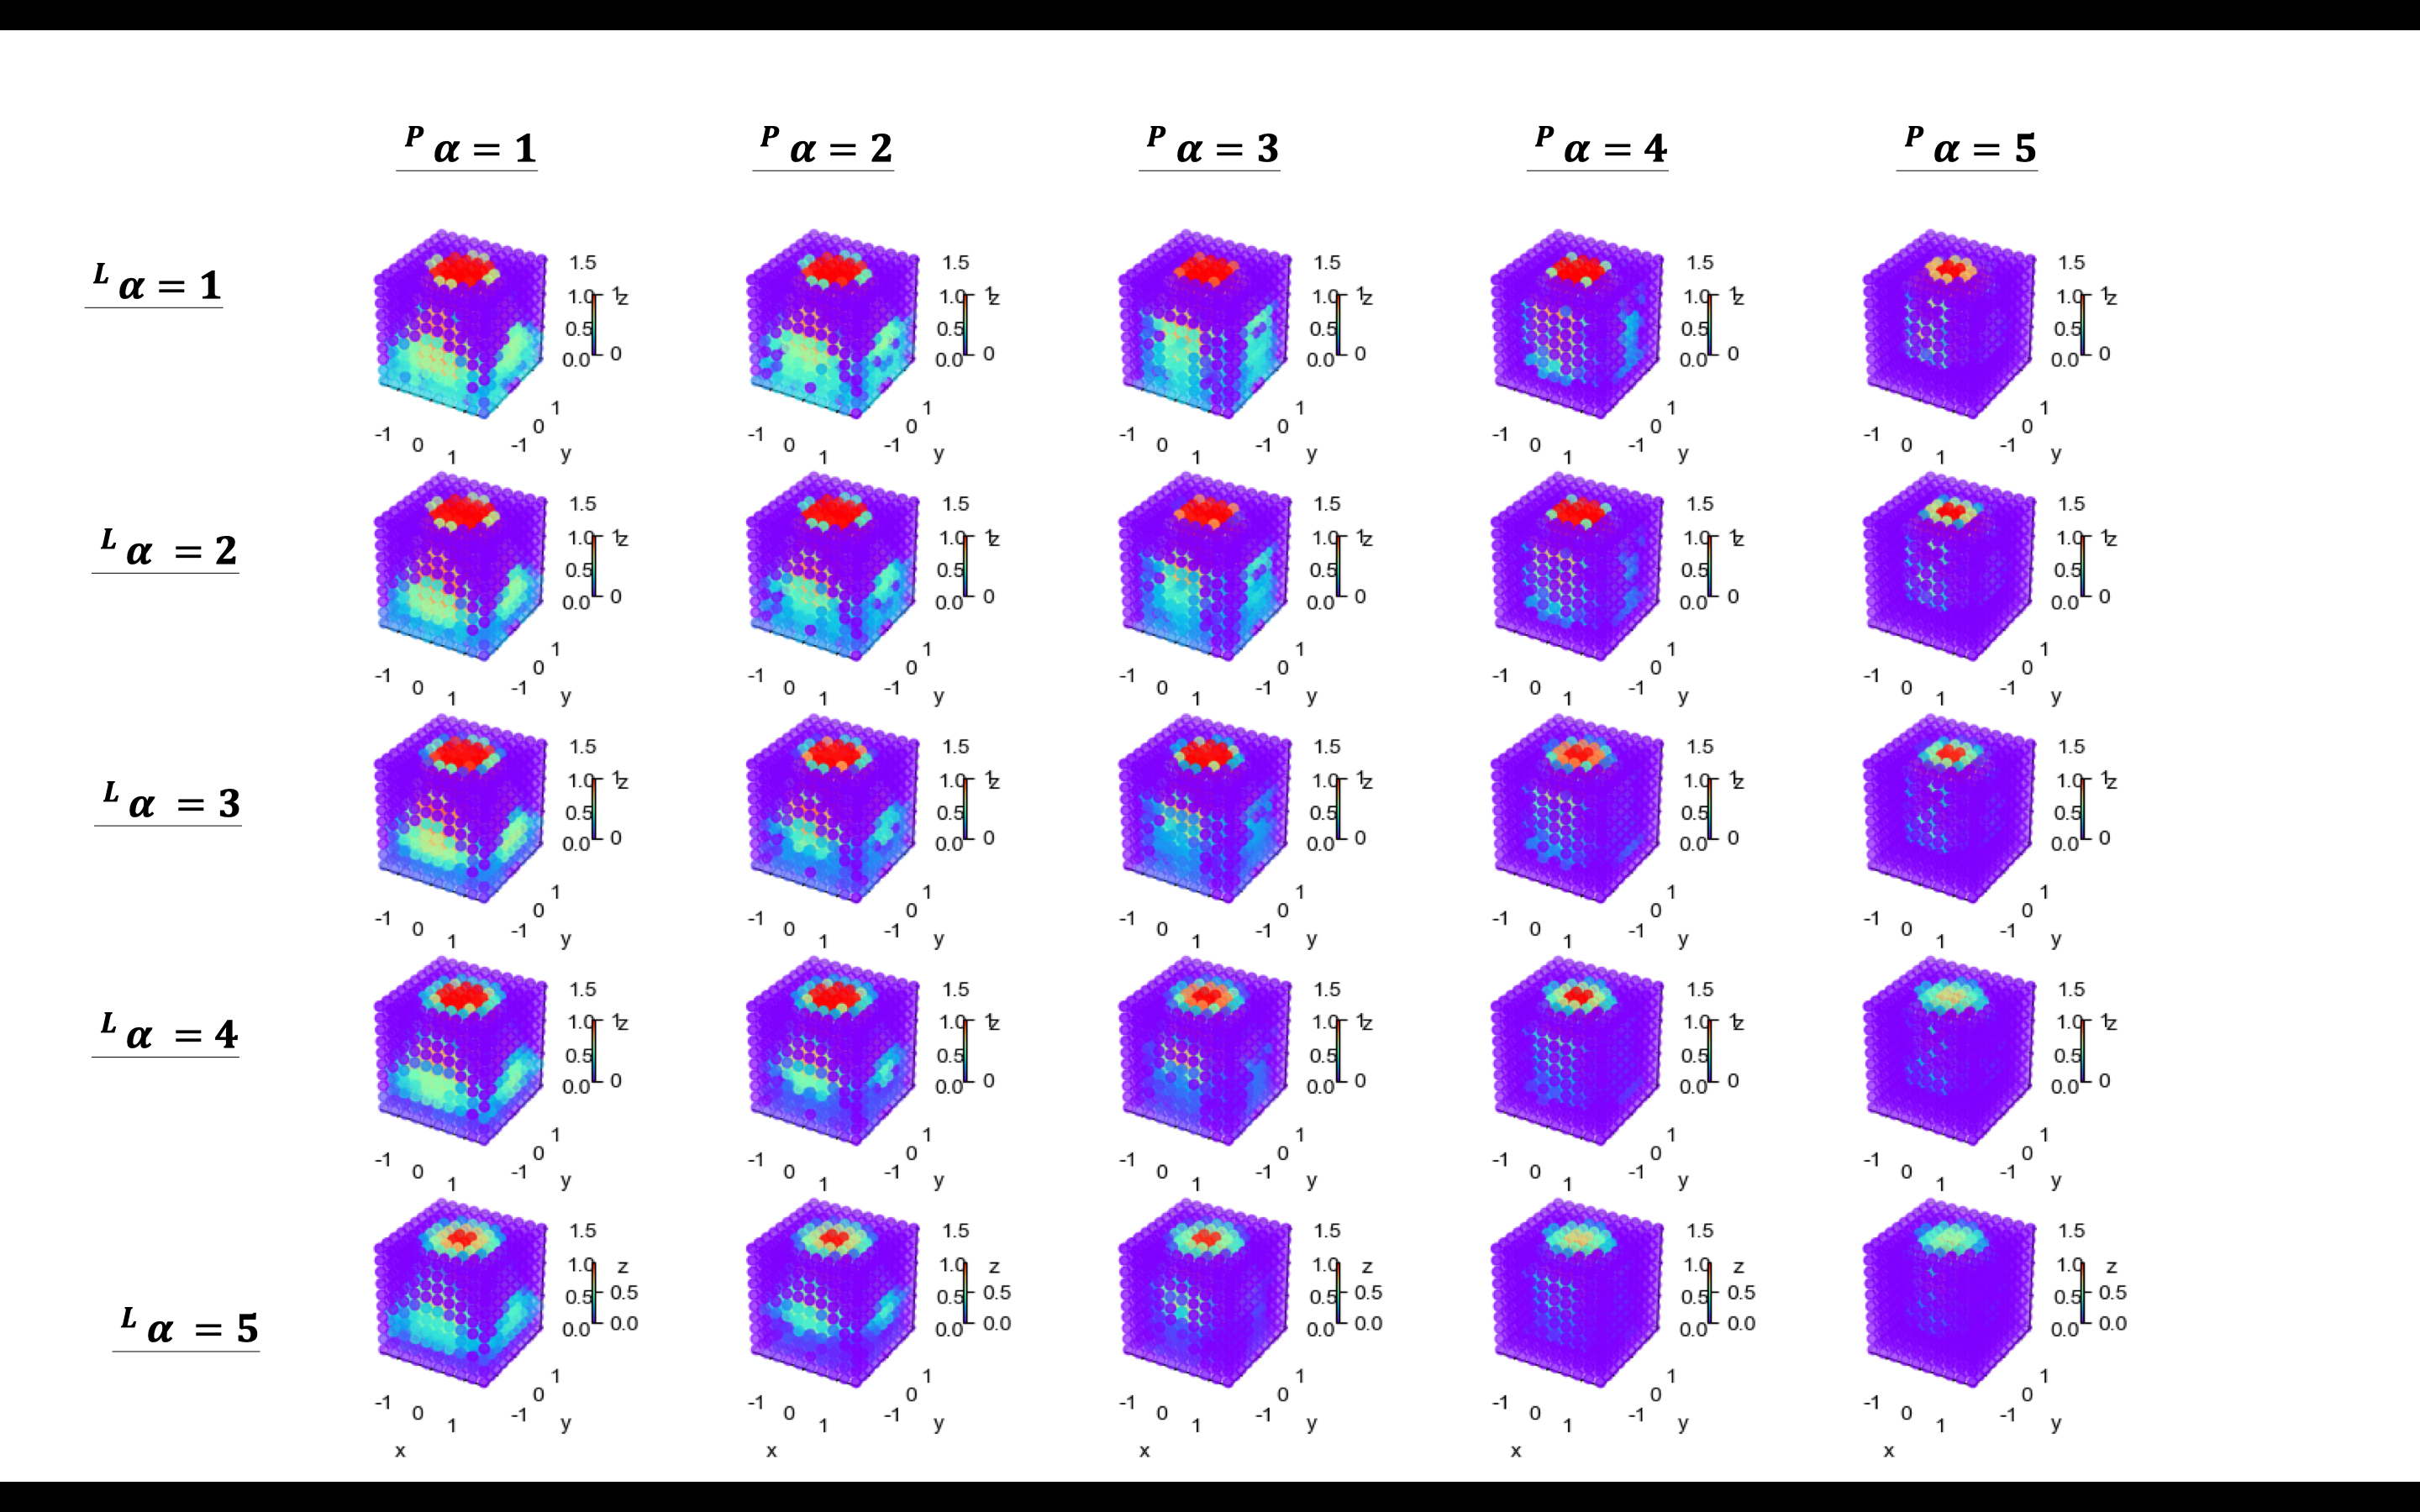
\includegraphics[width=14cm]{ch4pic/alpha_translate.png}
    \caption{改變硬體指向對平移樣本點的影響}
    \label{pic:alpha_translate}
\end{figure}
\begin{figure}[h!]
    \centering
    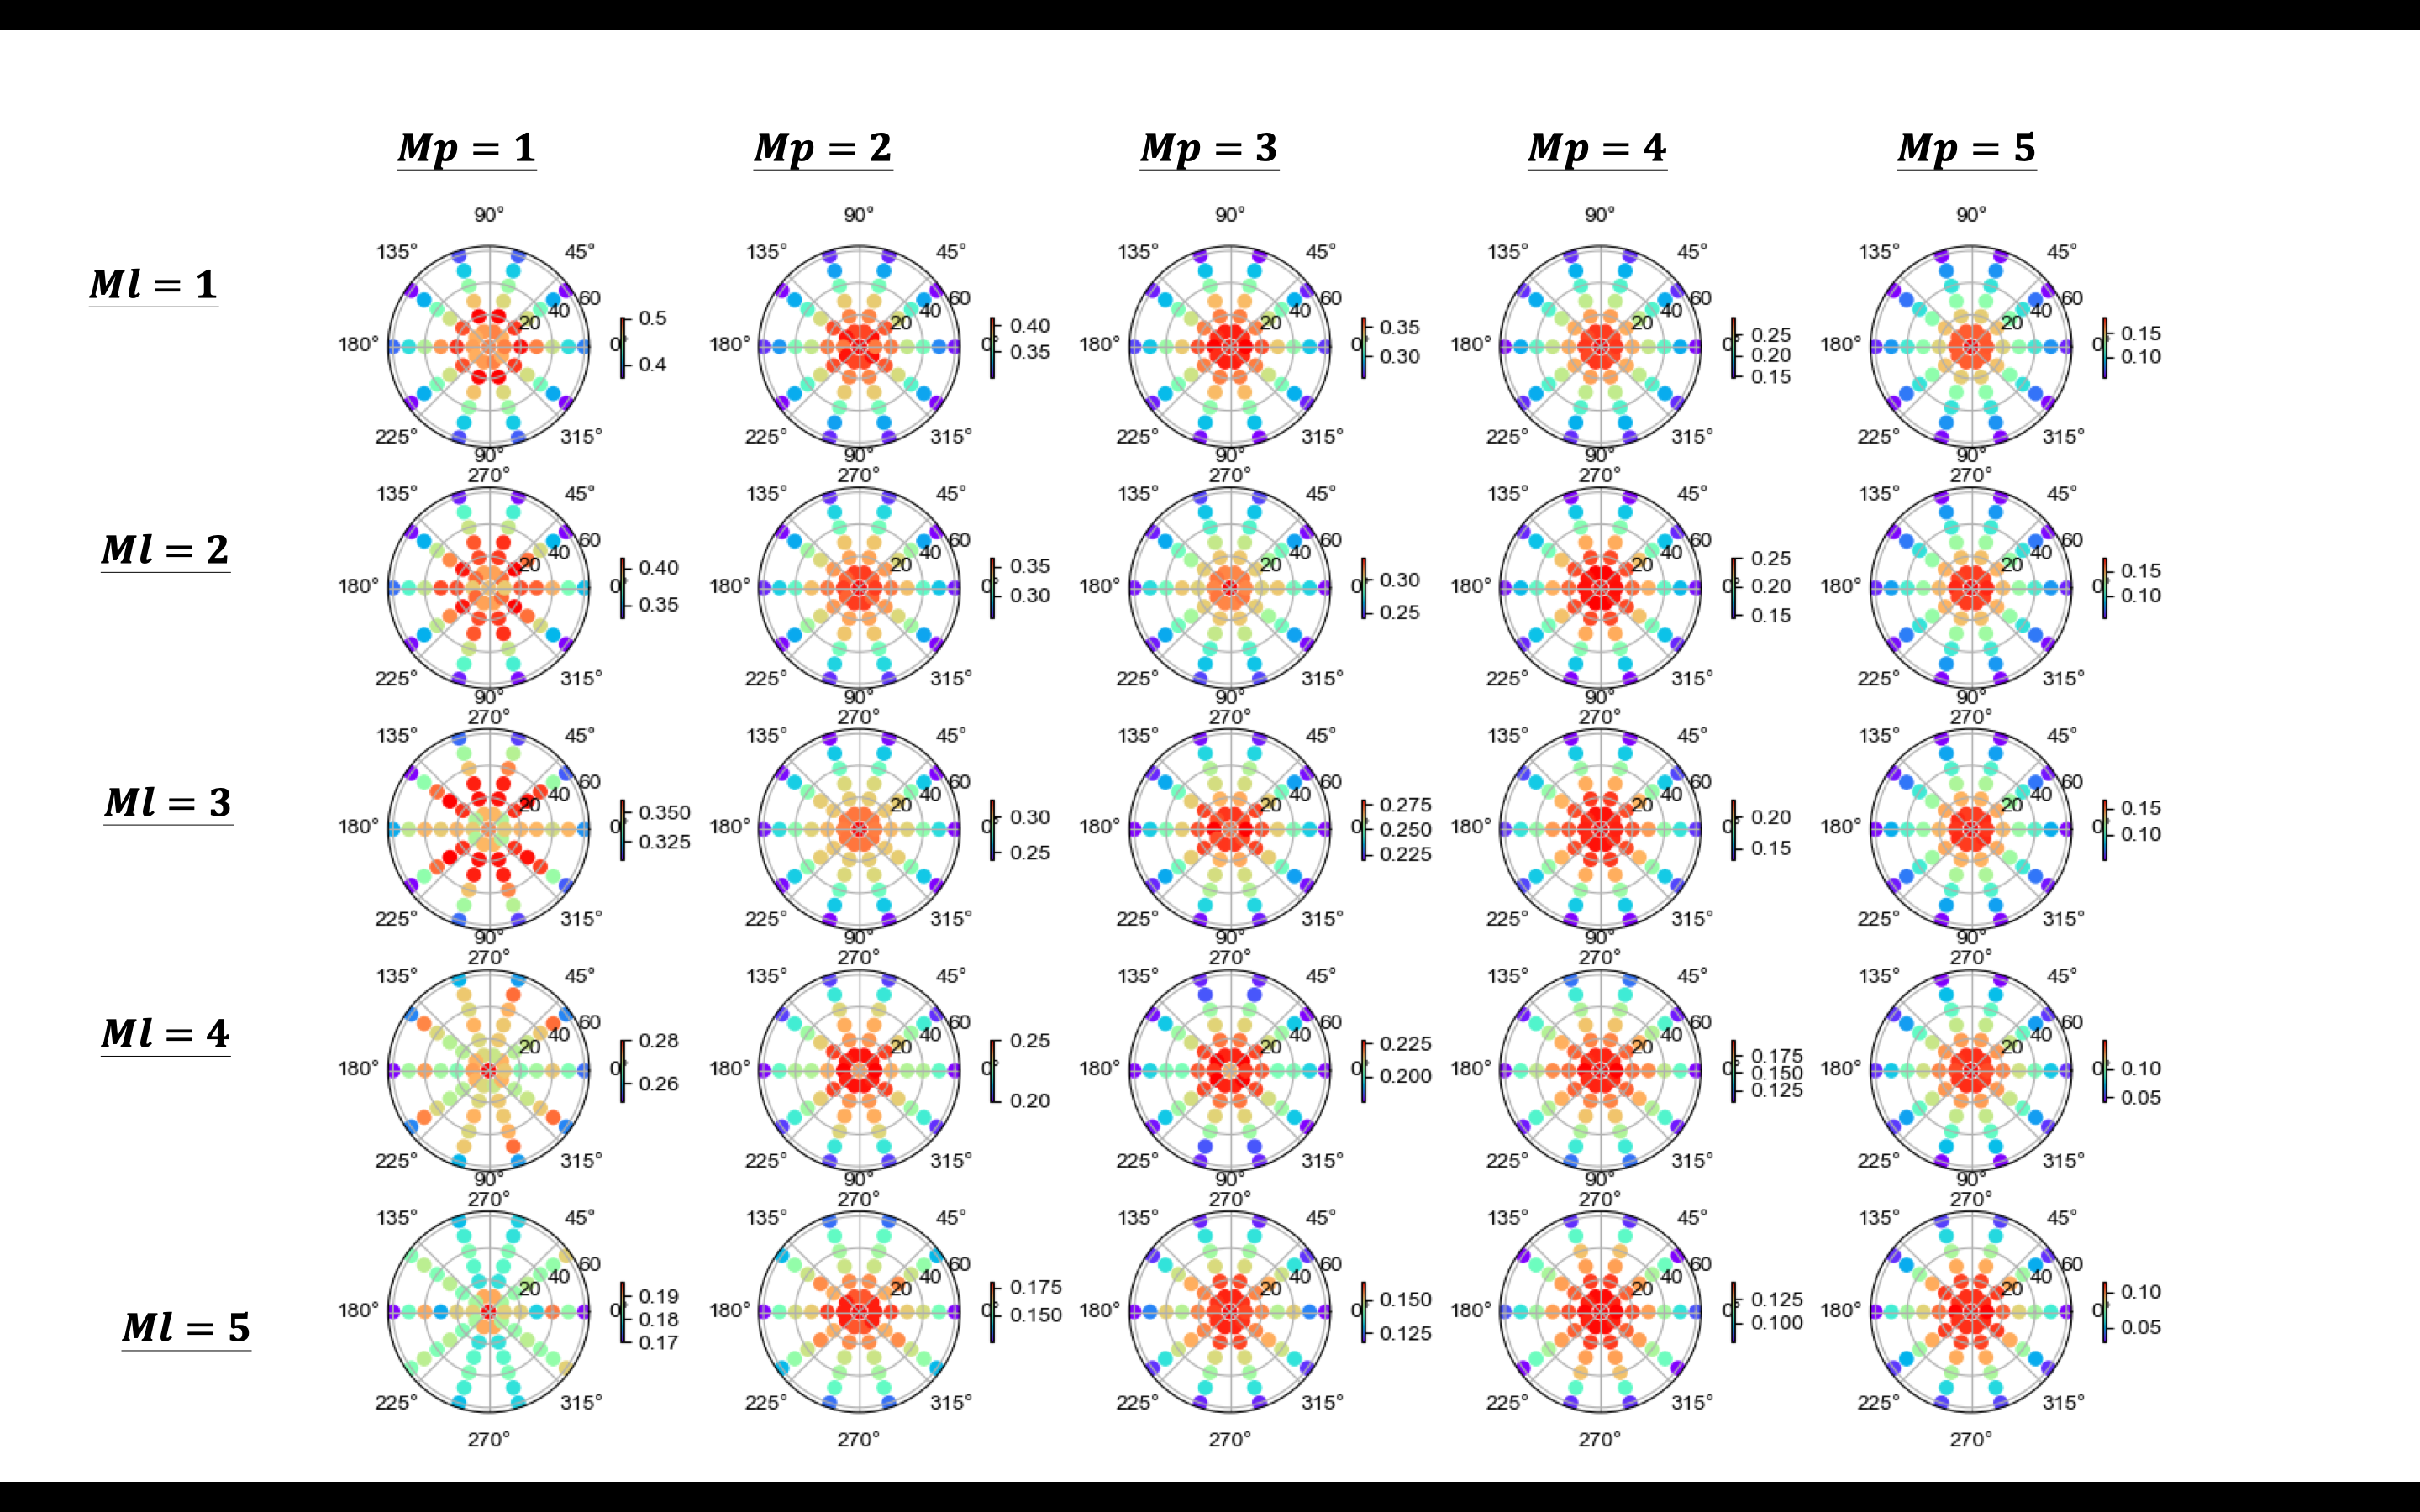
\includegraphics[width=14cm]{ch4pic/m_rotate.png}
    \caption{改變硬體指向對旋轉樣本點的影響}
    \label{pic:alpha_rotate}
\end{figure}

我們將平移與旋轉樣本點總共六萬個點中,在容許範圍內的比例,呈現於圖\ref{pic:alpha_effect},我們可以觀察到在此情境中,較小的硬體擺設天頂角,使系統表現較佳。

\begin{figure}[h!]
    \centering
    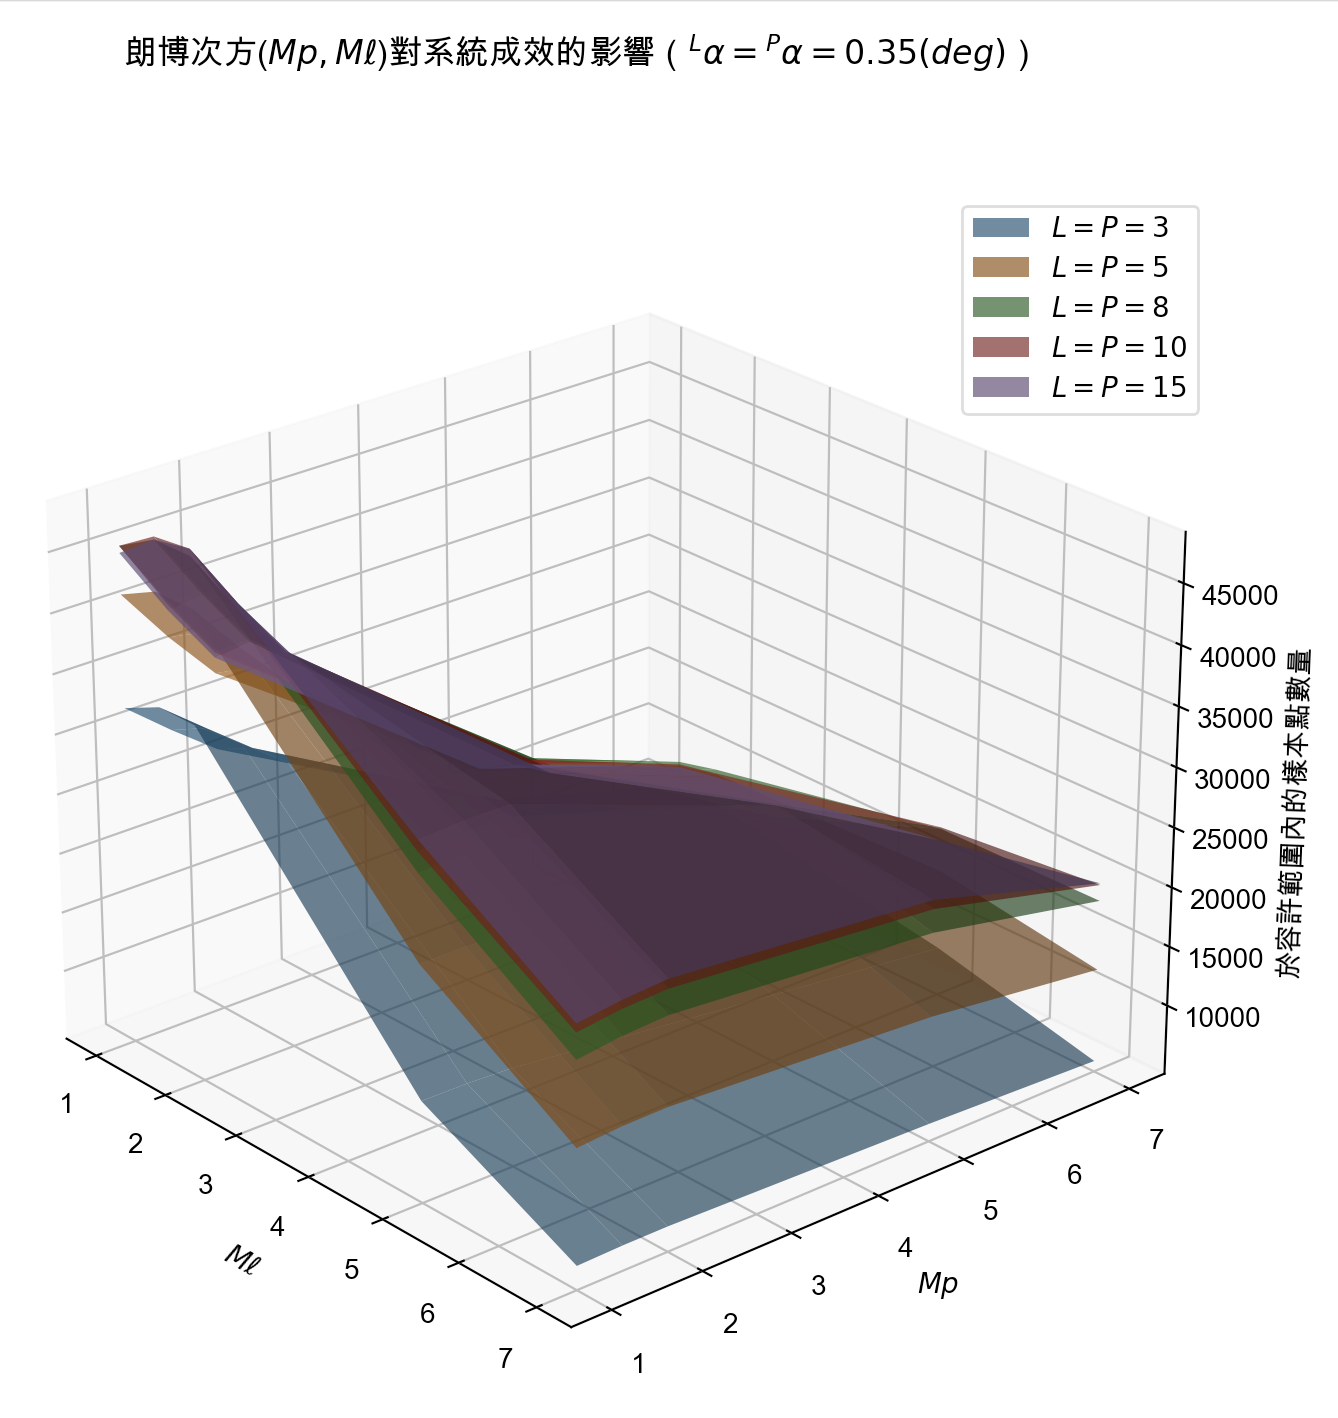
\includegraphics[width=9cm]{ch4pic/m_effect.png}
    \caption{改變硬體指向對系統的影響}
    \label{pic:alpha_effect}
\end{figure}



\subsection{LED與PD數量的影響}

由圖\ref{pic:m_effect}與圖\ref{pic:alpha_effect}中,我們都可以看出在提高硬體數量時,系統表現提升,然而系統表現提升的幅度不與硬體提升的數量成正比。因此,在挑選硬體數量時,除了系統表現以外,也需將硬體增加所造成的硬體成本,以及架設系統的難度考慮進來,在系統表現與硬體系統簡單中取捨。

% --------------------------------------
\section{結論}
\label{chp:4_conclusion}


由以上分析,我們可以看出在\ref{chp:scenario}章中提出的情境下,小的朗博次方與較小的硬體天頂角$\alpha$使系統的表現較佳,而硬體數量則是愈多愈好,但成長的趨勢隨著硬體數量增多而減慢。

我們本章節提出的方法,可以在軟體中透過改變硬體的選擇、樣本點的集合、組態等,快速的對不同情境,評估不同系統設計的表現。有了此模擬方法,我們可以在硬體系統架設之前對系統表現有所了解,避免在硬體架設的部分浪費時間與硬體成本。除此之外,藉由可以分析不同設計下的系統表現,我們進而於第五章針對不同情境,進行朗博次方、硬體指向以及硬體數量的最佳化,提供特定使用情境下的最佳系統設計。